%  !TeX  root  =  user_guide.tex

\chapter{GRASS GIS Integration}\label{sec:grass}\index{GRASS}

% when the revision of a section has been finalized,
% comment out the following line:
% \updatedisclaimer

The GRASS plugin provides access to GRASS GIS~\cite{GRASSweb} databases and
functionalities. This includes visualization of GRASS raster and vector
layers, digitizing vector layers, editing vector attributes, creating new
vector layers and analysing GRASS 2D and 3D data with more than 300 GRASS
modules.

In this Section we'll introduce the plugin functionalities and give some
examples on managing and working with GRASS data. Following main features
are provided with the toolbar menu, when you start the GRASS plugin, as
described in Section~\ref{sec:starting_grass}:

\begin{itemize}[label=--]
\item \toolbtntwo{grass_open_mapset}{Open mapset}
\item \toolbtntwo{grass_new_mapset}{New mapset}
\item \toolbtntwo{grass_close_mapset}{Close mapset}
\item \toolbtntwo{grass_add_vector}{Add GRASS vector layer}
\item \toolbtntwo{grass_add_raster}{Add GRASS raster layer}
\item \toolbtntwo{grass_new_vector_layer}{Create new GRASS vector}
\item \toolbtntwo{grass_edit}{Edit GRASS vector layer}
\item \toolbtntwo{grass_tools}{Open GRASS tools}
%\item \toolbtntwo{grass_shell}{Open GRASS Shell}
\item \toolbtntwo{grass_region}{Display current GRASS region}
\item \toolbtntwo{grass_region_edit}{Edit current GRASS region}
\end{itemize}

\section{Starting the GRASS plugin}\label{sec:starting_grass}
\index{GRASS!starting QGIS}

To use GRASS functionalities and/or visualize GRASS vector and raster layers
in QGIS, you must select and load the GRASS plugin with the Plugin Manager.
Therefore click the menu \mainmenuopt{Plugins} \arrow \mainmenuopt{Manage Plugins},
select \dropmenuopt{GRASS} and click \button{OK}.

You can now start loading raster and vector layers from an existing GRASS
\filename{LOCATION} (see Section \ref{sec:load_grassdata}). Or you create a
new GRASS \filename{LOCATION} with QGIS (see Section \ref{sec:create_loc})
and import some raster and vector data (see Section \ref{sec:import_loc_data})
for further analysis with the GRASS Toolbox (see Section
\ref{subsec:grass_toolbox}).

\section{Loading GRASS raster and vector layers}\label{sec:load_grassdata}\index{GRASS!loading data}

With the GRASS plugin, you can load vector or raster layers using the
appropriate button on the toolbar menu. As an example we use the QGIS alaska
dataset (see Section \ref{label_sampledata}). It includes a small sample
GRASS \filename{LOCATION} with 3 vector layers and 1 raster elevation map.

\begin{enumerate}
 \item Create a new folder \filename{grassdata}, download the QGIS alaska
  dataset \filename{qgis\_sample\_data.zip} from
  \url{http://download.osgeo.org/qgis/data/} and unzip the file into
  \filename{grassdata}.
  \item Start QGIS.
  \item If not already done in a previous QGIS session, load the GRASS plugin
  clicking on \mainmenuopt{Plugins} \arrow \mainmenuopt{Manage Plugins} and
  selecting \dropmenuopt{GRASS}. The GRASS toolbar appears on the toolbar menu.
  \item In the GRASS toolbar, click the \toolbtntwo{grass_open_mapset}{Open
  mapset} icon to bring up the \filename{MAPSET} wizard.
  \item For \filename{Gisdbase} browse and select or enter the path to the
  newly created folder \filename{grassdata}.
  \item You should now be able to select the \filename{LOCATION alaska}
  and the MAPSET \filename{demo}.
  \item Click \button{OK}. Notice that some previously disabled tools in the
  GRASS toolbar are now enabled.
  \item Click on \toolbtntwo{grass_add_raster}{Add GRASS raster layer},
  choose the map name \filename{gtopo30} and click \button{OK}. The elevation
  layer will be visualized.
  \item Click on \toolbtntwo{grass_add_vector}{Add GRASS vector layer},
  choose the map name \filename{alaska} and click \button{OK}. The alaska
  boundary vector layer will be overlayed on top of the \usertext{gtopo30} map. You can
  now adapt the layer properties as described in chapter \ref{sec:vectorprops},
  e.g. change opacity, fill and outline color.
  \item Also load the other two vector layers \filename{rivers} and
  \filename{airports} and adapt their properties.
\end{enumerate}

As you see, it is very simple to load GRASS raster and vector layers in QGIS.
See following Sections for editing GRASS data and creating a new
\filename{LOCATION}. More sample GRASS \filename{LOCATIONs} are available at
the GRASS website at \url{http://grass.osgeo.org/download/data.php}.

\begin{Tip}\caption{\textsc{GRASS Data Loading}}
If you have problems loading data or QGIS terminates abnormally,
check to make sure you have loaded the GRASS plugin properly as described in
Section \ref{sec:starting_grass}.
\end{Tip}

\section{GRASS LOCATION and MAPSET}\label{sec:about_loc}

GRASS data are stored in a directory referred to as GISDBASE. This directory
often called \filename{grassdata}, must be created before you start working
with the GRASS plugin in QGIS. Within this directory, the GRASS GIS data
are organized by projects stored in subdirectories called \filename{LOCATION}.
Each \filename{LOCATION} is defined by its coordinate system, map projection
and geographical boundaries. Each \filename{LOCATION} can have several
\filename{MAPSETs} (subdirectories of the \filename{LOCATION}) that are used
to subdivide the project into different topics, subregions, or as workspaces
for individual team members (Neteler \& Mitasova 2008
\cite{neteler_mitasova08}). In order to analyze vector and raster layers with
GRASS modules, you must import them into a GRASS \filename{LOCATION}.
\footnote{This is not strictly true - with the GRASS modules
\filename{r.external} and \filename{v.external} you can create read-only links
to external GDAL/OGR-supported data sets without importing them. But because
this is not the usual way for beginners to work with GRASS, this functionality
will not be described here.}

\begin{figure}[ht]
\centering
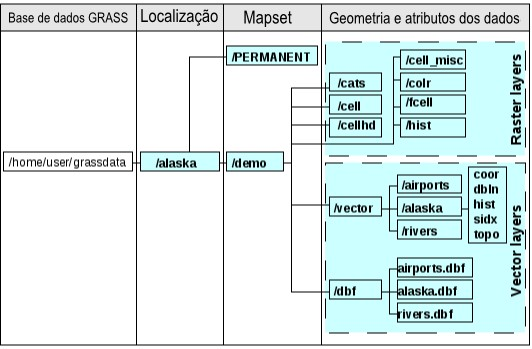
\includegraphics[clip=true]{grass_location}
\caption{GRASS data in the alaska LOCATION (adapted from Neteler \& Mitasova 2008 \cite{neteler_mitasova08})}\label{fig:grass_location}\end{figure}

\subsection{Creating a new GRASS LOCATION}\label{sec:create_loc}

As an example here is how the sample GRASS
\filename{LOCATION alaska}, which is projected in Albers Equal Area
projection with unit feet was created for the QGIS sample dataset. This
sample GRASS \filename{LOCATION alaska} will be used for all examples and
exercises in the following GRASS GIS related chapters. It is useful to
download and install the dataset on your computer \ref{label_sampledata}).

\begin{figure}[ht]
\centering
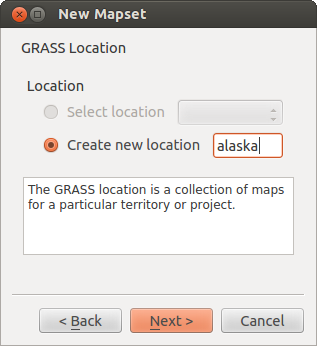
\includegraphics[clip=true, width=8cm]{create_grass_location}
\caption{Creating a new \grass LOCATION or a new MAPSET in \qg \nixcaption}
\label{fig:create_grass_location}
\end{figure}

\begin{enumerate}
  \item Start QGIS and make sure the GRASS plugin is loaded
  \item Visualize the \filename{alaska.shp} Shapefile (see Section
  \ref{sec:load_shapefile}) from the QGIS alaska dataset~\ref{label_sampledata}.
  \item In the GRASS toolbar, click on the \toolbtntwo{grass_open_mapset}{Open
    mapset} icon to bring up the \filename{MAPSET} wizard.
  \item Select an existing GRASS database (GISDBASE) folder
  \filename{grassdata} or create one for the new \filename{LOCATION} using a
  file manager on your computer. Then click \button{Next}.
  \item We can use this wizard to create a new \filename{MAPSET} within an
  existing \filename{LOCATION} (see Section~\ref{sec:add_mapset}) or to create
  a new \filename{LOCATION} altogether. Click on the radio button
  \radiobuttonon{Create new location} (see Figure \ref{fig:create_grass_location}).
  \item Enter a name for the \filename{LOCATION} - we used alaska and click
  \button{Next}
  \item Define the projection by clicking on the radio button
  \radiobuttonon{Projection} to enable the projection list
  \item We are using Albers Equal Area Alaska (feet) projection. Since we
  happen to know that it is represented by the EPSG ID 2964, we enter it in
  the search box. (Note: If you want to repeat this process for another
  \filename{LOCATION} and projection and haven't memorized the EPSG ID,
  click on the
  \toolbtntwo{mIconProjectionEnabled}{projector} icon in the lower right-hand
  corner of the status bar (see Section \ref{label_projstart})).
  \item Click \button{Find} to select the projection
  \item Click \button{Next}
  \item To define the default region, we have to enter the \filename{LOCATION}
  bounds in north, south, east, and west direction. Here we simply click on
  the button \button{Set current QGIS extent}, to apply the extend of the
  loaded layer \filename{alaska.shp} as the GRASS default region extend.
  \item Click \button{Next}
  \item We also need to define a \filename{MAPSET} within our new
  \filename{LOCATION}. You can name it whatever you like - we used demo.
  \footnote{When creating a new \filename{LOCATION}, GRASS automatically
  creates a special \filename{MAPSET} called \filename{PERMANENT} designed to
  store the core data for the project, its default spatial extend and
  coordinate system definitions (Neteler \& Mitasova 2008
  \cite{neteler_mitasova08}).}
  \item Check out the summary to make sure it's correct and click
  \button{Finish}
  \item The new \filename{LOCATION alaska} and two \filename{MAPSETs demo}
  and \filename{PERMANENT} are created. The currently opened working set is
  \filename{MAPSET demo}, as you defined.
  \item Notice that some of the tools in the GRASS toolbar that were
  disabled are now enabled.
\end{enumerate}

If that seemed like a lot of steps, it's really not all that bad and a very
quick way to create a \filename{LOCATION}. The \filename{LOCATION alaska} is
now ready for data import (see Section \ref{sec:import_loc_data}).
You can also use the already existing vector and raster data in the sample
GRASS \filename{LOCATION alaska} included in the QGIS alaska dataset
\ref{label_sampledata} and move on to Section \ref{label_vectmodel}.

\subsection{Adding a new MAPSET}\label{sec:add_mapset}

A user has only write access to a GRASS \filename{MAPSET} he created. This
means that besides access to his own \filename{MAPSET}, each user can read
maps in other user's \filename{MAPSETs}, but he can modify or remove only
the maps in his own \filename{MAPSET}. All \filename{MAPSETs} include a
\filename{WIND} file that stores the current boundary coordinate values and
the currently selected raster resolution (Neteler \& Mitasova 2008
\cite{neteler_mitasova08}, see Section \ref{sec:grass_region}).

\begin{enumerate}
  \item Start QGIS and make sure the GRASS plugin is loaded
  \item In the GRASS toolbar, click on the
  \toolbtntwo{grass_new_mapset}{New mapset} icon to bring up the
  \filename{MAPSET} wizard.
  \item Select the GRASS database (GISDBASE) folder \filename{grassdata}
  with the \filename{LOCATION alaska}, where we want to add a further
  \filename{MAPSET}, called test.
  \item Click \button{Next}.
  \item We can use this wizard to create a new \filename{MAPSET} within an
  existing \filename{LOCATION} or to create a new \filename{LOCATION}
  altogether. Click on the radio button \radiobuttonon{Select location}
  (see Figure \ref{fig:create_grass_location}) and click \button{Next}.
  \item Enter the name \filename{text} for the new \filename{MAPSET}. Below
  in the wizard you see a list of existing \filename{MAPSETs} and its owners.
  \item Click \button{Next}, check out the summary to make sure it's all
  correct and click \button{Finish}
\end{enumerate}

\section{Importing data into a GRASS LOCATION}\label{sec:import_loc_data}

This Section gives an example how to import raster and vector data into the
\filename{alaska} GRASS \filename{LOCATION} provided by the QGIS alaska
dataset. Therefore we use a landcover raster map \filename{landcover.img}
and a vector GML File \filename{lakes.gml} from the QGIS alaska
dataset \ref{label_sampledata}.

\begin{enumerate}
  \item Start QGIS and make sure the GRASS plugin is loaded.
  \item In the GRASS toolbar, click the \toolbtntwo{grass_open_mapset}{Open
  MAPSET} icon to bring up the \filename{MAPSET} wizard.
  \item Select as GRASS database the folder \filename{grassdata} in the QGIS
  alaska dataset, as \filename{LOCATION alaska}, as \filename{MAPSET}
  \filename{demo} and click \button{OK}.
  \item Now click the \toolbtntwo{grass_tools}{Open GRASS tools} icon. The
  GRASS Toolbox (see Section \ref{subsec:grass_toolbox}) dialog appears.
  \item To import the raster map \filename{landcover.img}, click the module
  \filename{r.in.gdal} in the \tab{Modules Tree} tab. This GRASS module
  allows to import GDAL supported raster files into a GRASS
  \filename{LOCATION}. The module dialog for \filename{r.in.gdal} appears.
  \item Browse to the folder \filename{raster} in the QGIS alaska dataset
  and select the file \filename{landcover.img}.
  \item As raster output name define \filename{landcover\_grass} and click
  \button{Run}. In the \tab{Output} tab you see the currently running GRASS
  command \filename{r.in.gdal -o input=/path/to/landcover.img
  output=landcover\_grass}.
  \item When it says \textbf{Succesfully finished} click \button{View output}.
  The \filename{landcover\_grass} raster layer is now imported into GRASS and
  will be visualized in the QGIS canvas.
  \item To import the vector GML file \filename{lakes.gml}, click the module
  \filename{v.in.ogr} in the \tab{Modules Tree} tab. This GRASS module allows
  to import OGR supported vector files into a GRASS \filename{LOCATION}. The
  module dialog for \filename{v.in.ogr} appears.
  \item Browse to the folder \filename{gml} in the QGIS alaska
  dataset and select the file \filename{lakes.gml} as OGR file.
  \item As vector output name define \filename{lakes\_grass} and click
  \button{Run}. You don't have to care about the other options in this
  example. In the \tab{Output} tab you see the currently running GRASS
  command \filename{v.in.ogr -o dsn=/path/to/lakes.gml output=lakes\_grass}.
  \item When it says \textbf{Succesfully finished} click \button{View output}.
  The \filename{lakes\_grass} vector layer is now imported into GRASS and will
  be visualized in the QGIS canvas.
\end{enumerate}


\section{The GRASS vector data model}\label{label_vectmodel}\index{GRASS!vector data
model}

It is important to understand the GRASS vector data model prior to
digitizing.\index{GRASS!digitizing} In general, GRASS uses a topological
vector model.\index{GRASS!topology} This means that areas are not represented
as closed polygons, but by one or more boundaries. A boundary between two
adjacent areas is digitized only once, and it is shared by both areas.
Boundaries must be connected and closed without gaps. An area is identified (and labeled)
by the \textbf{centroid} of the area.

Besides boundaries and centroids, a vector map can also contain
points and lines. All these geometry elements can be mixed
in one vector and will be represented in different so called 'layers' inside
one GRASS vector map. So in GRASS a layer is not a vector or raster map but a
level inside a vector layer. This is important to distinguish carefully.
\footnote{Although it
is possible to mix geometry elements, it is unusual and even in GRASS only
used in special cases such as vector network analysis. Normally you should
prefere to store different geometry elements in different layers.}

It is possible to store several 'layers' in one vector dataset. For example,
fields, forests and lakes can be stored in one vector. Adjacent
forest and lake can share the same boundary, but they have separate attribute
tables. It is also possible to attach attributes to boundaries. For example,
the boundary between lake and forest is a road, so it can have a different
attribute table.

The 'layer' of the feature is defined by 'layer' inside GRASS. 'Layer' is the
number which defines if there are more than one layer inside the dataset, e.g.
if the geometry is forest or lake. For now, it can be only a number, in the
future GRASS will also support names as fields in the user interface.

Attributes can be stored inside the GRASS \filename{LOCATION} as DBase or
SQLITE3 or in external database tables, for example PostgreSQL, MySQL,
Oracle, etc.\index{GRASS!attribute storage}

Attributes in database tables are linked to geometry elements using
a 'category' value.\index{GRASS!attribute linkage} 'Category' (key, ID) is an
integer attached to geometry primitives, and it is used as the link to one
key column in the database table.

\begin{Tip}\caption{\textsc{Learning the GRASS Vector Model}}
The best way to learn the GRASS vector model and its capabilities is to
download one of the many GRASS tutorials where the vector model is described
more deeply. See \url{http://grass.osgeo.org/gdp/manuals.php} for more
information, books and tutorials in several languages.
\end{Tip}

\section{Creating a new GRASS vector layer}\label{sec:creating_new_grass_vectors}\index{GRASS!Creating new vectors|see{editing!creating a new layer}}

To create a new GRASS vector layer with the GRASS plugin click the
\toolbtntwo{grass_new_vector_layer}{Create new GRASS vector} toolbar icon.
Enter a name in the text box and you can start digitizing point, line or
polygon geometries, following the procedure described in Section
\ref{grass_digitizing}.

In GRASS it is possible to organize all sort of geometry types (point, line
and area) in one layer, because GRASS uses a topological vector model, so you
don't need to select the geometry type when creating a new GRASS vector. This
is different from Shapefile creation with QGIS, because Shapefiles use the
Simple Feature vector model (see Section \ref{sec:create shape}).

\begin{Tip}\caption{\textsc{Creating an attribute table for a new GRASS vector layer}}
If you want to assign attributes to your digitized geometry features, make sure to create an attribute table with columns before you start digitizing (see Figure \ref{fig:grass_digitizing_table}).
\end{Tip}

\section{Digitizing and editing a GRASS vector layer}\index{GRASS!digitizing tools}\label{grass_digitizing}

The digitizing tools for GRASS vector layers are accessed using the
\toolbtntwo{grass_edit}{Edit GRASS vector layer} icon on the toolbar. Make
sure you have loaded a GRASS vector and it is the selected layer in the legend
before clicking on the edit tool. Figure \ref{fig:grass_digitizing_category}
shows the GRASS edit dialog that is displayed when you click on the edit tool.
The tools and settings are discussed in the following sections.

\begin{Tip}\caption{\textsc{Digitizing polygons in GRASS}}
If you want to create a polygon in GRASS, you first digitize the boundary of
the polygon, setting the mode to \usertext{No category}. Then you add a
centroid (label point) into the closed boundary, setting the mode to
\usertext{Next not used}. The reason is, that a topological vector model links
attribute information of a polygon always to the centroid and not to the
boundary.
\end{Tip}

\minisec{Toolbar}\label{label_grasstoolbar}

In Figure \ref{fig:grass_digitizing_toolbar} you see the GRASS digitizing
toolbar icons provided by the GRASS plugin. Table \ref{tab:grass_tools}
explains the available functionalities.

\begin{figure}[h]
   \centering
   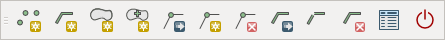
\includegraphics[clip=true,width=12cm]{grass_digitizing_toolbar}
   \caption{GRASS Digitizing Toolbar \nixcaption}\label{fig:grass_digitizing_toolbar}
\end{figure}

{\renewcommand{\arraystretch}{2}
\begin{table}[h]\index{GRASS!digitizing tools}
\centering
 \begin{tabular}{|m{1cm}|m{4cm}|m{8.5cm}|}
 \hline \textbf{Icon} & \textbf{Tool} & \textbf{Purpose} \\
\hline 
\includegraphics[width=0.7cm]{grass_new_point} & New Point & Digitize
new point \\
\hline 
\includegraphics[width=0.7cm]{grass_new_line} & New Line & Digitize
new line (finish by selecting new tool) \\
\hline 
\includegraphics[width=0.7cm]{grass_new_boundary} & New Boundary &
Digitize new boundary (finish by selecting new tool)\\
\hline 
\includegraphics[width=0.7cm]{grass_new_centroid} & New Centroid &
Digitize new centroid (label existing area)\\
\hline 
\includegraphics[width=0.7cm]{grass_move_vertex} & Move vertex & Move
one vertex of existing line or boundary and identify new position\\
\hline 
\includegraphics[width=0.7cm]{grass_add_vertex} & Add vertex & Add a
new vertex to existing line\\
\hline 
\includegraphics[width=0.7cm]{grass_delete_vertex} & Delete vertex &
Delete vertex from existing line (confirm selected vertex by another click)\\
\hline 
\includegraphics[width=0.7cm]{grass_move_line} & Move element & Move
selected boundary, line, point or centroid and click on new position\\
\hline 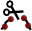
\includegraphics[width=0.7cm]{grass_split_line} & Split line & Split
an existing line to 2 parts\\
\hline 
\includegraphics[width=0.7cm]{grass_delete_line} & Delete element &
Delete existing boundary, line, point or centroid (confirm selected element by
another click)\\
\hline 
\includegraphics[width=0.7cm]{grass_edit_attributes} & Edit attributes
& Edit attributes of selected element (note that one element can represent
more features, see above)\\
\hline 
\includegraphics[width=0.7cm]{grass_close_edit} & Close & Close
session and save current status (rebuilds topology afterwards)\\
\hline
\end{tabular}
\caption{GRASS Digitizing Tools}\label{tab:grass_tools}
\end{table}}

\minisec{Category Tab}\index{GRASS!category settings}

The \tab{Category} tab allows you to define the way in which the category
values will be assigned to a new geometry element.

\begin{figure}[h]
 \centering
  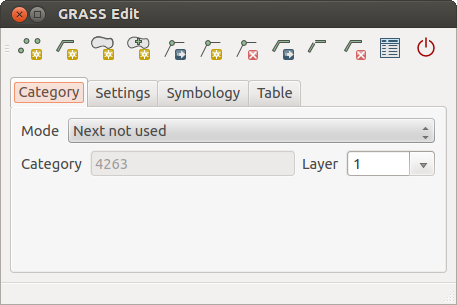
\includegraphics[clip=true,width=8cm]{grass_digitizing_category}
  \caption{GRASS Digitizing Category Tab \nixcaption}\label{fig:grass_digitizing_category}
 \end{figure}

\begin{itemize}[label=--]
\item \textbf{Mode}: what category value shall be applied to new geometry
elements.
\begin{itemize}[label=--]
\item Next not used - apply next not yet used category value to geometry
element.
\item Manual entry - manually define the category value for the geometry
element in the 'Category'-entry field.
\item No category - Do not apply a category value to the geometry element.
This is e.g. used for area boundaries, because the category values are
connected via the centroid.
\end{itemize}
\item \textbf{Category} - A number (ID) is attached to each digitized geometry
element. It is used to connect each geometry element with its attributes.
\item \textbf{Field (layer)} - Each geometry element can be connected with
several attribute tables using different GRASS geometry layers. Default layer
number is 1.
\end{itemize}

\begin{Tip}\caption{\textsc{Creating an additional GRASS 'layer' with QGIS}}
If you would like to add more layers to your dataset, just add a new
number in the 'Field (layer)' entry box and press return. In the Table tab
you can create your new table connected to your new layer.
\end{Tip}

\minisec{Settings Tab}\label{label_settingtab}\index{GRASS!snapping
tolerance}

The \tab{Settings} tab allows you to set the snapping in screen pixels. The
threshold defines at what distance new points or line ends are snapped to
existing nodes. This helps to prevent gaps or dangles between boundaries. The
default is set to 10 pixels.

\begin{figure}[h]
 \centering
 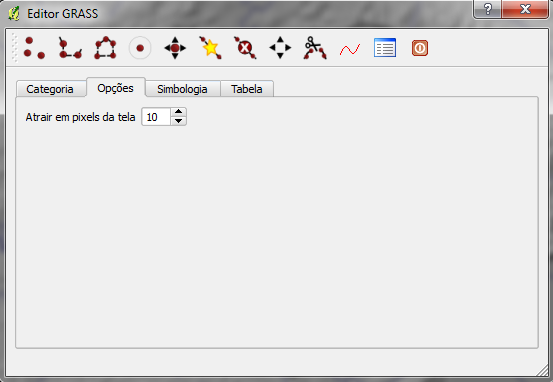
\includegraphics[clip=true,width=8cm]{grass_digitizing_settings}
 \caption{GRASS Digitizing Settings Tab \nixcaption}\label{fig:grass_digitizing_settings}
\end{figure}

\minisec{Symbology Tab}\index{GRASS!symbology settings}

The \tab{Symbology} tab allows you to view and set symbology and color
settings for various geometry types and their topological status (e.g. closed
/ opened boundary).

\begin{figure}[h]
 \centering
 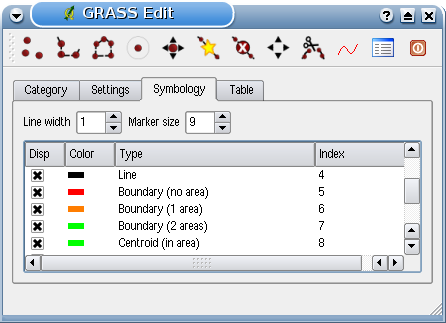
\includegraphics[clip=true,width=8cm]{grass_digitizing_symbology}
 \caption{GRASS Digitizing Symbolog Tab \nixcaption}\label{fig:grass_digitizing_symbology}
\end{figure}

\minisec{Table Tab} \index{GRASS!table editing}

The \tab{Table} tab provides information about the database table for
a given 'layer'. Here you can add new columns to an existing attribute table,
or create a new database table for a new GRASS vector layer (see Section
\ref{sec:creating_new_grass_vectors}).

\begin{figure}[h]
 \centering
 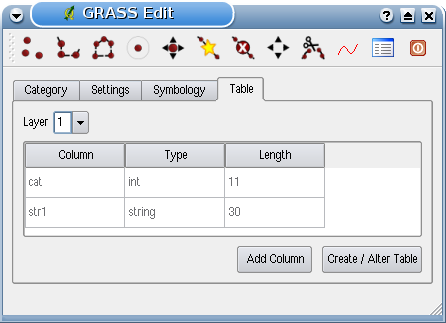
\includegraphics[clip=true,width=10cm]{grass_digitizing_table}
 \caption{GRASS Digitizing Table Tab \nixcaption}\label{fig:grass_digitizing_table}
 \end{figure}

\begin{Tip}\caption{\textsc{GRASS Edit Permissions}}\index{GRASS!edit
permissions}
You must be the owner of the GRASS \filename{MAPSET} you want to
edit. It is impossible to edit data layers in a \filename{MAPSET} that is not
yours, even if you have write permissions.
\end{Tip}

\section{The GRASS region tool}\label{sec:grass_region}\index{GRASS!region}

The region definition (setting a spatial working window) in GRASS is important
for working with raster layers. Vector analysis is by default not limited
to any defined region definitions. But all newly-created rasters will have the
spatial extension and resolution of the currently defined GRASS region,
regardless of their original extension and resolution. The current GRASS
region is stored in the \filename{\$LOCATION/\$MAPSET/WIND} file, and it
defines north, south, east and west bounds, number of columns and rows,
horizontal and vertical spatial resolution.

It is possible to switch on/off the visualization of the GRASS region in the
QGIS canvas using the \toolbtntwo{grass_region}{Display current GRASS region}
button. \index{GRASS!region!display}.

With the \toolbtntwo{grass_region_edit}{Edit current GRASS region} icon you
can open a dialog to change the current region and the symbology of the GRASS
region rectangle in the QGIS canvas. Type in the new region bounds and
resolution and click \button{OK}. It also allows to select a new region
interactively with your mouse on the QGIS canvas. Therefore click with the
left mouse button in the QGIS canvas, open a rectangle, close it using the
left mouse button again and click \button{OK}.\index{GRASS!region!editing}
The GRASS module \filename{g.region} provide a lot more parameters to define
an appropriate region extend and resolution for your raster analysis. You can
use these parameters with the GRASS Toolbox, described in Section
\ref{subsec:grass_toolbox}.

\section{The GRASS toolbox}\label{subsec:grass_toolbox}\index{GRASS!toolbox}

The \toolbtntwo{grass_tools}{Open GRASS Tools} box provides GRASS module
functionalities to work with data inside a selected GRASS \filename{LOCATION}
and \filename{MAPSET}. To use the GRASS toolbox you need to open a
\filename{LOCATION} and \filename{MAPSET} where you have write-permission
(usually granted, if you created the \filename{MAPSET}). This is necessary,
because new raster or vector layers created during analysis need to be written
to the currently selected \filename{LOCATION} and \filename{MAPSET}.

The GRASS Shell inside the GRASS Toolbox provides access to almost all (more
than 330) GRASS modules through a command line interface. To offer a more user
friendly working environment, about 200 of the available GRASS modules and
functionalities are also provided by graphical dialogs within the GRASS plugin Toolbox.

\subsection{Working with GRASS modules}\label{grass_modules}\index{GRASS!toolbox}

\begin{figure}[ht]
\centering
   \subfloat[Modules Tree] {\label{subfig:grass_module_tree}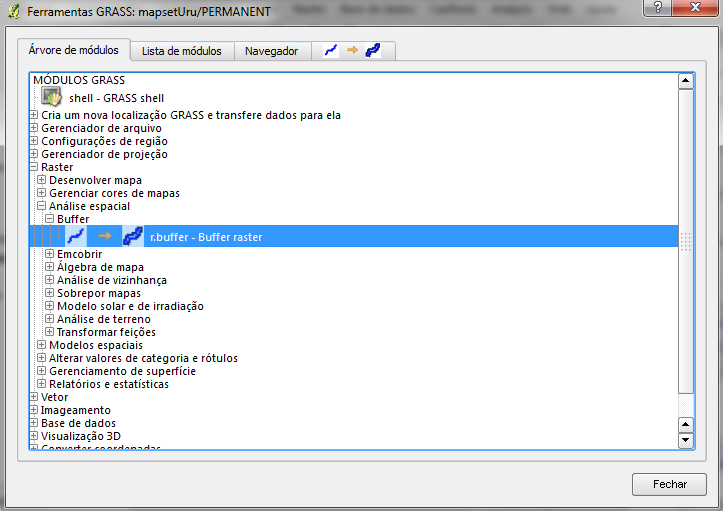
\includegraphics[clip=true, width=0.4\textwidth]{grass_toolbox_moduletree}}
   \hspace{0.5cm}
   \subfloat[Searchable Modules List] {\label{subfig:grass_module_list}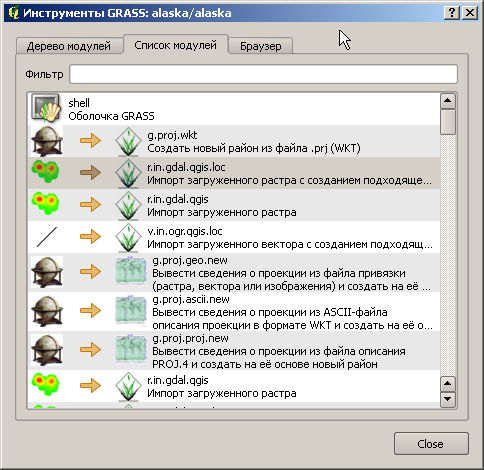
\includegraphics[clip=true, width=0.4\textwidth]{grass_toolbox_modulelist}}
\caption{GRASS Toolbox and searchable Modules List \nixcaption}\label{fig:grass_modules}
\end{figure}

The GRASS Shell inside the GRASS Toolbox provides access to almost all (more
than 300) GRASS modules in a command line interface. To offer a more user
friendly working environment, about 200 of the available GRASS modules and
functionalities are also provided by graphical dialogs. These dialogs are
grouped in categories, but are searchable as well. 

A complete list of GRASS modules available in the graphical Toolbox in QGIS version \CURRENT
is available in the GRASS wiki ( \url{http://grass.osgeo.org/wiki/GRASS-QGIS_relevant_module_list}. 

It is also possible to customize the GRASS Toolbox content. This procedure is described in Section
\ref{sec:toolbox-customizing}.

As shown in Figure \ref{fig:grass_modules}, you can look for the appropriate
GRASS module using the thematically grouped \tab{Modules Tree} or the
searchable \tab{Modules List} tab.

Clicking on a grapical module icon a new tab will be added to the toolbox
dialog providing three new sub-tabs \tab{Options}, \tab{Output} and
\tab{Manual}. In Figure \ref{fig:grass_module_dialog} you see an example
for the GRASS module \filename{v.buffer}.

\begin{figure}[h]
\centering
   \subfloat[Module Options] {\label{subfig:grass_module_option}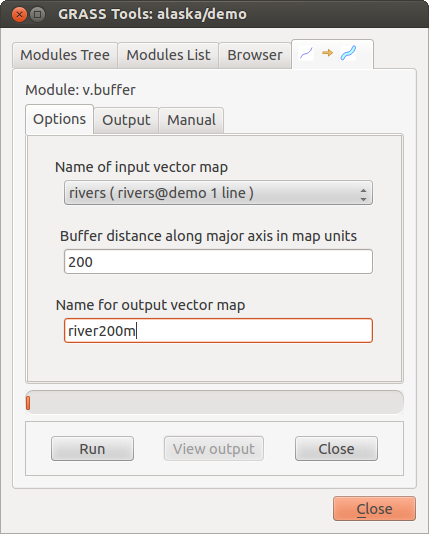
\includegraphics[clip=true, width=0.3\textwidth]{grass_module_option}}
   \hspace{1cm}
   \subfloat[Modules Output] {\label{subfig:grass_module_output}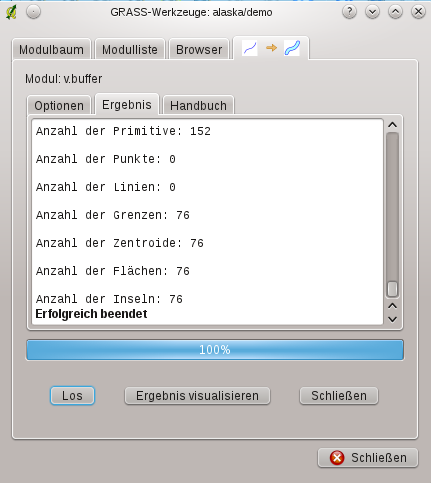
\includegraphics[clip=true, width=0.3\textwidth]{grass_module_output}}
   \hspace{1cm}
   \subfloat[Module Manual] {\label{subfig:grass_module_manual}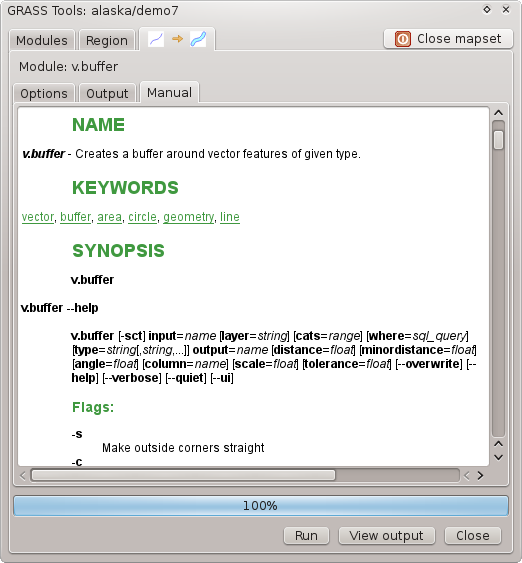
\includegraphics[clip=true, width=0.3\textwidth]{grass_module_manual}}
\caption{GRASS Toolbox Module Dialogs \nixcaption}\label{fig:grass_module_dialog}
\end{figure}
\FloatBarrier
\minisec{Options}

The \tab{Options} tab provides a simplified module dialog where you can
usually select a raster or vector layer visualized in the QGIS canvas and
enter further module specific parameters to run the module. The provided
module parameters are often not complete to keep the dialog clear. If you want
to use further module parameters and flags, you need to start the GRASS Shell
and run the module in the command line.

A new feature in QGIS \CURRENT is the support for a
\button{show advanced options >>} button below the simplified module dialog
in the \tab{Options} tab. At the moment it is only added to the module v.in.ascii
as an example use, but will probably be part of more / all modules in the
GRASS toolbox in future versions of QGIS. This allows to use the complete GRASS
module options without the need to switch to the GRASS Shell.

\minisec{Output}

The \tab{Output} tab provides information about the output status of the
module. When you click the \button{Run} button, the module switches to the
\tab{Output} tab and you see information about the analysis process. If all
works well, you will finally see a \usertext{Successfully finished} message.

\minisec{Manual}

The \tab{Manual} tab shows the HTML help page of the GRASS module. You can
use it to check further module parameters and flags or to get a deeper
knowledge about the purpose of the module. At the end of each module
manual page you see further links to the \filename{Main Help index}, the
\filename{Thematic index} and the \filename{Full index}. These links provide
the same information as if you use the module \filename{g.manual}

\begin{Tip}\caption{\textsc{Display results immediately}}\index{GRASS!display results}
If you want to display your calculation results immediately in your
map canvas, you can use the 'View Output' button at the bottom of the
module tab.
\end{Tip}

\subsection{GRASS module examples}\index{GRASS!toolbox}
The following examples will demonstrate the power of some of the GRASS modules.

\minisec{Creating contour lines}

The first example creates a vector contour map from an elevation raster
(DEM). Assuming you have the Alaska \filename{LOCATION} set up as explained
in Section \ref{sec:import_loc_data}.

\begin{itemize}[label=--]
\item First open the location by clicking the
\toolbtntwo{grass_open_mapset}{Open mapset} button and choosing the Alaska
location.
\item Now load the \usertext{gtopo30} elevation raster by clicking
\toolbtntwo{grass_add_raster}{Add GRASS raster layer} and selecting the
\usertext{gtopo30} raster from the demo location.
\item Now open the Toolbox with the \toolbtntwo{grass_tools}{Open GRASS
tools} button.
\item In the list of tool categories double click Raster \arrow Surface
Management \arrow Generate vector contour lines.
\item Now a single click on the tool \classname{r.contour} will open
the tool dialog as explained above \ref{grass_modules}. The
\usertext{gtopo30} raster should appear as the \inputtext{Name of input
raster}{gtopo30}.
\item Type into the \inputtext{Increment between Contour levels}{100} the
value 100. (This will create contour lines at intervals of
100 meters.)
\item Type into the \inputtext{Name for output vector map}{ctour\_100}
the name \usertext{ctour\_100}.
\item Click \button{Run} to start the process. Wait for several moments until
the message \usertext{Successfully finished} appears in the output window.
Then click \button{View Output} and \button{close}.
\end{itemize}

\begin{figure}[ht]
\centering
   \subfloat[r.contour Options] {\label{subfig:grass_toolbox_rcontour}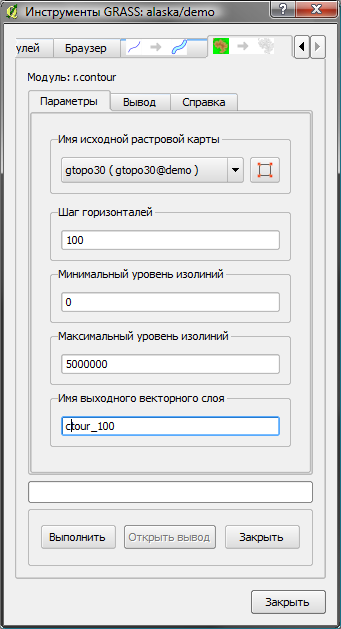
\includegraphics[clip=true, width=0.4\textwidth]{grass_toolbox_rcontour}}
    \hspace{0.5cm}
   \subfloat[r.contour Output] {\label{subfig:grass_toolbox_rcontour2}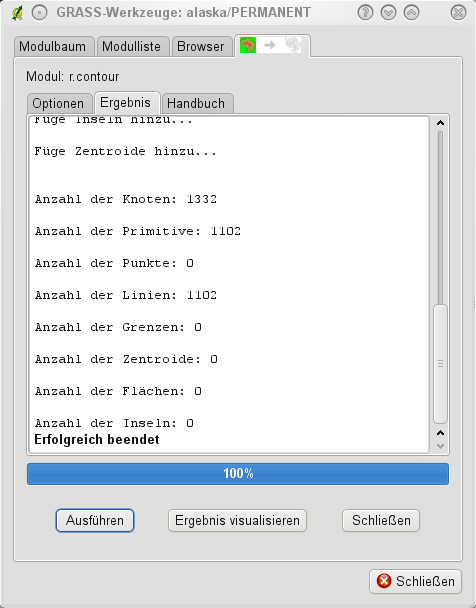
\includegraphics[clip=true, width=0.4\textwidth]{grass_toolbox_rcontour2}}
   \caption{\grass Toolbox r.contour module \nixcaption}\label{fig:grass_toolbox_rcontour}
\end{figure}

Since this is a large region, it will take a while to display. After it
finishes rendering, you can open the layer properties window to change the
line color so that the contours appear clearly over the elevation raster, as
in \ref{sec:vectorprops}.

Next zoom in to a small mountainous area in the center of Alaska.
Zooming in close you will notice that the contours have sharp corners. GRASS
offers the \classname{v.generalize} tool to slightly alter vector maps while
keeping their overall shape. The tool uses several different algorithms with
different purposes. Some of the algorithms (i.e. Douglas Peuker and Vertex
reduction) simplify the line by removing some of the vertices. The resulting
vector will load faster. This process will be used when you have a highly
detailed vector, but you are creating a very small scale map, so the detail
is unnecessary.

\begin{Tip}\caption{\textsc{The simplify tool}}\index{GRASS!display results}
Note that the QGIS fTools plugin has a \dropmenuopt{Simplify
geometries} tool that works just like the GRASS \classname{v.generalize}
Douglas-Peuker algorithm.
\end{Tip}

However, the purpose of this example is different. The contour lines created
by r.contour have sharp angles that should be smoothed. Among the
\classname{v.generalize} algorithms there is Chaikens which does just that
(also Hermite splines). Be aware that these algorithms can \textbf{add}
additional vertices to the vector, causing it to load even more slowly.

\begin{itemize}[label=--]
\item Open the GRASS toolbox and double click the categories Vector \arrow
Develop map \arrow Generalization, then click on the \classname{v.generalize}
module to open its options window.
\item Check that the \usertext{ctour\_100} vector appears as the
\inputtext{Name of input vector}{ctour\_100}.
\item From the list of algorithms choose Chaiken's. Leave all other options
at their default, and scroll down to the last row to enter the
\inputtext{Name for output vector map}{ctour\_100\_smooth}, and click
\button{Run}.
\item The process takes several moments. Once \usertext{Successfully
finished} appears in the output windows, click \button{View output} and then
\button{close}.
\item You may change the color of the vector to display it clearly on the
raster background and to contrast with the original contour lines. You will
notice that the new contour lines have smoother corners than the original
while staying faithful to the original overall shape.
\end{itemize}

\begin{figure}[h]
 \centering
 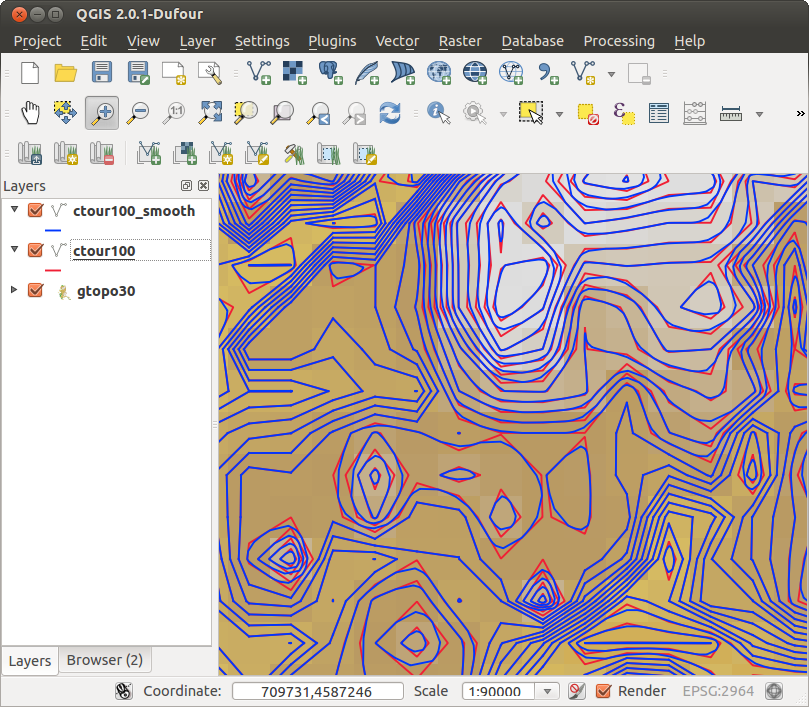
\includegraphics[clip=true, width=14cm]{grass_toolbox_vgeneralize}
 \caption{GRASS module v.generalize to smooth a vector map \nixcaption}\label{fig:grass_toolbox_vgeneralize}
\end{figure}

\begin{Tip}\caption{\textsc{Other uses for r.contour}}\index{GRASS!toolbox}
The procedure described above can be used in other equivalent
situations. If you have a raster map of precipitation data, for example, then
the same method will be used to create a vector map of isohyetal (constant
rainfall) lines
\end{Tip}

\minisec{Creating a Hillshade 3D effect}

Several methods are used to display elevation layers and give a 3D effect to
maps. The use of contour lines as shown above is one popular method often
chosen to produce topographic maps. Another way to display a 3D effect is by
hillshading. The hillshade effect is created from a DEM (elevation) raster by
first calculating the slope and aspect of each cell, then simulating the
sun's position in the sky and giving a reflectance value to each cell. Thus
you get sun facing slopes lighted and the slopes facing away from the sun (in
shadow) are darkened.

\begin{itemize}[label=--]
\item Begin this example by loading the \usertext{gtopo30} elevation raster.
Start the GRASS toolbox and under the Raster category double click to open Spatial
analysis \arrow Terrain analysis.
\item Then click \classname{r.shaded.relief} to open
the module.
\item Change the \inputtext{azimuth angle}{270} to 315. Enter
\usertext{gtopo30\_shade} for the new hillshade raster, and click
\button{run}.
\item When the process completes, add the hillshade raster to the map. You
should see it displayed in grayscale.
\item To view both the hill shading and the colors of the
\usertext{gtopo30} together shift the hillshade map below the
\usertext{gtopo30} map in the table of contents, then open the
\dropmenuopt{Properties} window of \usertext{gtopo30}, switch to the
\tab{transparency} tab and set its transparency level to about 25\%.
\end{itemize}

You should now have the \usertext{gtopo30} elevation with its colormap and
transparency setting displayed \textbf{above} the grayscale hillshade map. In
order to see the visual effects of the hillshading, turn off the
\usertext{gtopo30\_shade} map, then turn it back on.

\minisec{Using the GRASS shell}

The GRASS plugin in QGIS is designed for users who are new to GRASS, and not
familiar with all the modules and options. As such, some modules in the
toolbox do not show all the options available, and some modules do not appear
at all. The GRASS shell (or console) gives the user access to those
additional GRASS modules that do not appear in the toolbox tree, and also to
some additional options to the modules that are in the toolbox with the
simplest default parameters. This example demonstrates the use of an
additional option in the \classname{r.shaded.relief} module that was shown
above.

\begin{figure}[ht]
 \centering
 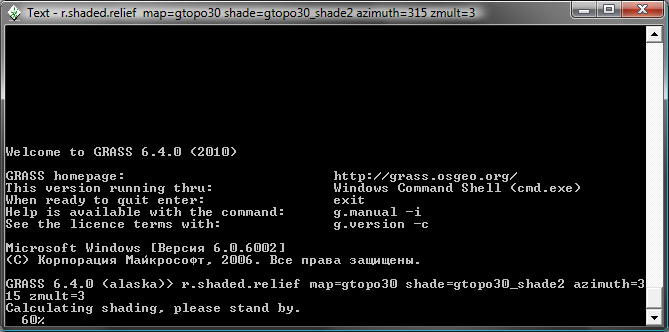
\includegraphics[clip=true, width=12cm]{grass_toolbox_shell}
 \caption{The GRASS shell, r.shaded.relief module \nixcaption}\label{fig:grass_toolbox_shell}
\end{figure}

The module \classname{r.shaded.relief} can take a parameter \usertext{zmult}
which multiplies the elevation values relative to the X-Y coordinate units so
that the hillshade effect is even more pronounced.

\begin{itemize}[label=--]
\item Load the \usertext{gtopo30} elevation raster as above, then start the
GRASS toolbox and click on the GRASS shell. In the shell window type the
command:\linebreak
\usertext{r.shaded.relief map=gtopo30 shade=gtopo30\_shade2 azimuth=315
zmult=3} \linebreak and press \keystroke{Enter}.
\end{itemize}

\begin{itemize}[label=--]
\item After the process finishes shift to the \tab{Browse} tab and double click on
the new \usertext{gtopo30\_shade2} raster to display in QGIS.
\item As explained above, shift the shaded relief raster below the gtopo30
raster in the Table of Contents, then check transparency of the colored
gtopo30 layer. You should see that the 3D effect stands out more strongly
compared to the first shaded relief map.
\end{itemize}

\begin{figure}[ht]
 \centering
 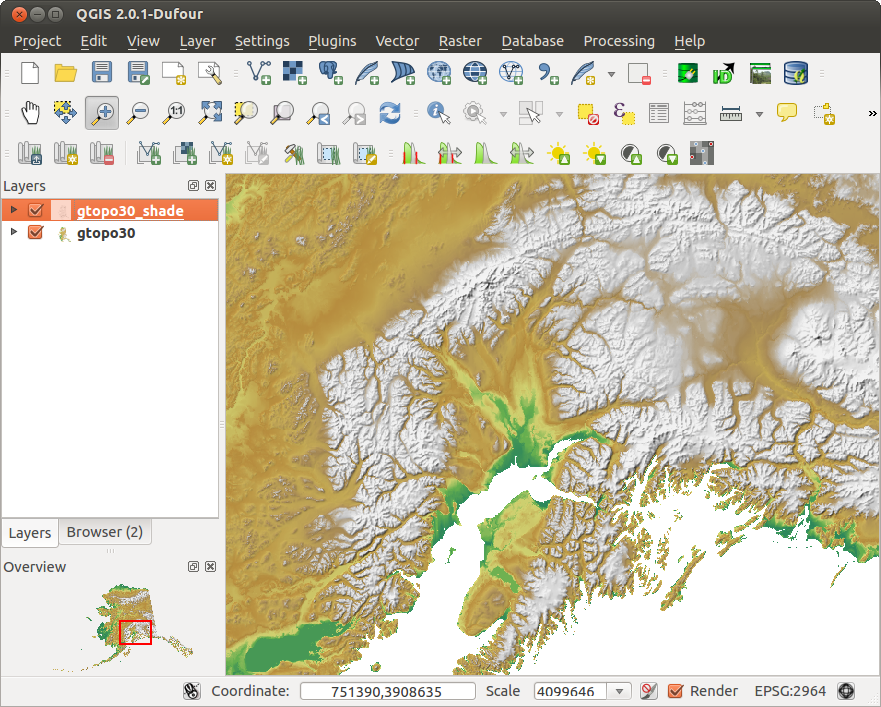
\includegraphics[clip=true, width=12cm]{grass_toolbox_shadedrelief}
 \caption{Displaying shaded relief created with the GRASS module
r.shaded.relief \nixcaption}\label{fig:grass_toolbox_shadedrelief}
\end{figure}

\minisec{Raster statistics in a vector map}

The next example shows how a GRASS module can aggregate raster data and add
columns of statistics for each polygon in a vector map.

\begin{itemize}[label=--]
\item Again using the Alaska data, refer to \ref{sec:import_loc_data} to
import the trees shapefile from the \usertext{shapefiles} directory
into GRASS.
\item Now an intermediary step is required: centroids must be added to the
imported trees map to make it a complete GRASS area vector (including both
boundaries and centroids).
\item From the toolbox choose Vector \arrow Manage features, and open the
module \classname{v.centroids}.
\item Enter as the \inputtext{output vector map}{\usertext{forest\_areas}}
and run the module.
\item Now load the \usertext{forest\_areas} vector and display the types of
forests - deciduous, evergreen, mixed - in different colors: In the layer
\dropmenuopt{Properties} window, \tab{symbology} tab, choose \\
\selectstring{Legend type}{Unique value} and set the
\inputtext{Classification field}{VEGDESC} to VEGDESC. (Refer to the
explanation of the symbology tab \ref{sec:symbology} in the vector section).
\item Next reopen the GRASS toolbox and open Vector \arrow Vector update by other
maps.
\item Click on the \classname{v.rast.stats} module. Enter \usertext{gtopo30},
and \usertext{forest\_areas}.
\item Only one additional parameter is needed: Enter \inputtext{column
prefix}{\usertext{elev}}, and click \button{run}. This is a computationally
heavy operation which will run for a long time (probably up to two hours).
\item Finally open the \usertext{forest\_areas} attribute table, and verify
that several new columns have been added including \usertext{elev\_min},
\usertext{elev\_max}, \usertext{elev\_mean} etc. for each forest polygon.
\end{itemize}

\subsection{Working with the GRASS LOCATION browser} \index{GRASS!toolbox!Browser}

Another useful feature inside the GRASS Toolbox is the GRASS
\filename{LOCATION} browser. In Figure~\ref{fig:grass_mapset_browser} you
can see the current working \filename{LOCATION} with its \filename{MAPSETs}.

In the left browser windows you can browse through all \filename{MAPSETs}
inside the current \filename{LOCATION}. The right browser window shows some
meta information for selected raster or vector layers, e.g. resolution,
bounding box, data source, connected attribute table for vector data and a
command history.

\begin{figure}[h]
 \centering
 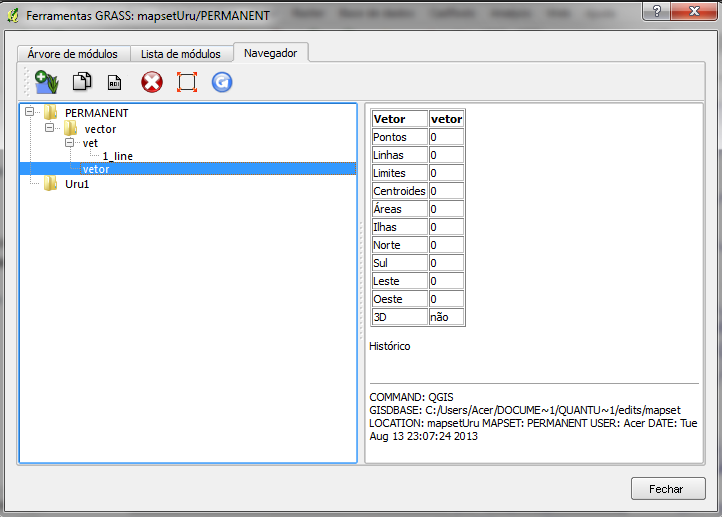
\includegraphics[clip=true,width=10cm]{grass_mapset_browser}
 \caption{GRASS LOCATION browser \nixcaption}\label{fig:grass_mapset_browser}
\end{figure}

The toolbar inside the \tab{Browser} tab offers following tools to manage
the selected \filename{LOCATION}:

\begin{itemize}[label=--]
\item \toolboxtwo{grass_add_map}{Add selected map to canvas}
\item \toolboxtwo{grass_copy_map}{Copy selected map}
\item \toolboxtwo{grass_rename_map}{Rename selected map}
\item \toolboxtwo{grass_delete_map}{Delete selected map}
\item \toolboxtwo{grass_set_region}{Set current region to selected map}
\item \toolboxtwo{grass_refresh}{Refresh browser window}
\end{itemize}

The \toolboxtwo{grass_rename_map}{Rename selected map} and
\toolboxtwo{grass_delete_map}{Delete selected map} only work with maps inside
your currently selected \filename{MAPSET}. All other tools also work with
raster and vector layers in another \filename{MAPSET}.

\subsection{Customizing the GRASS Toolbox} \index{GRASS!toolbox!customize}
\label{sec:toolbox-customizing}

Nearly all GRASS modules can be added to the GRASS toolbox. A XML
interface is provided to parse the pretty simple XML files which configures
the modules appearance and parameters inside the toolbox.

A sample XML file for generating the module \usertext{v.buffer} (v.buffer.qgm)
looks like this:
\begin{verbatim}
<?xml version="1.0" encoding="UTF-8"?>
<!DOCTYPE qgisgrassmodule SYSTEM "http://mrcc.com/qgisgrassmodule.dtd">

<qgisgrassmodule label="Vector buffer" module="v.buffer">
        <option key="input" typeoption="type" layeroption="layer" />
        <option key="buffer"/>
        <option key="output" />
</qgisgrassmodule>
\end{verbatim}

The parser reads this definition and creates a new tab inside the toolbox
when you select the module. A more detailed description for adding new
modules, changing the modules group, etc. can be found on the QGIS wiki at \\
\url{http://wiki.qgis.org/qgiswiki/Adding\_New\_Tools\_to\_the\_GRASS\_Toolbox}.

\FloatBarrier
